\documentclass{article}
\usepackage{polski}
\usepackage{blindtext}
\usepackage{amsmath}
\usepackage{mathtools}
\usepackage{graphicx} 
\usepackage{wrapfig}
\usepackage{amssymb}
\usepackage{multirow}
\usepackage[usenames,dvipsnames,svgnames,table]{xcolor}
\usepackage{float}
\usepackage[caption = false]{subfig}
\usepackage{caption}
\newcommand\tab[1][1cm]{\hspace*{#1}}
\usepackage[a4paper, left=2cm, right=2cm, top=2cm, bottom=2cm, headsep=1.2cm]{geometry}

\usepackage{titling}
\newcommand{\subtitle}[1]{%
  \posttitle{%
    \par\end{center}
    \begin{center}\large#1\end{center}
    \vskip0.5em}%
}


\title{Aproksymacja wielomianowa}
\author{Wiktoria Zaczyk}
\date{06.05.2021}

\usepackage{natbib}
\usepackage{graphicx}
\graphicspath{ {./images/} }

\begin{document}

\maketitle

\section{Wstęp teoretyczny}

\newline\newline
\textbf{Aproksymacja}:
\newline
Proces określania rozwiązań przybliżonych na podstawie rozwiązań 
znanych, które są bliskie rozwiązaniom dokładnym w ściśle sprecyzowanym sensie.
\newline\newline
\textbf{Aproksymacja liniowa funkcji}
\newline
Wyznaczenie współczynników ($a_0,a_1,a_2,...,a_m$) 
funkcji aproksymującej $F(x)=a_0\varphi_0(x)+a_1\varphi_1(x)+...+ a_m\varphi_m(x) $, gdzie: $\varphi_i(x)$ - są funkcjami bazowymi $(m+1)$ wymiarowej podprzestrzeni liniowej. Aby uzyskać bardzo dobre przybliżenie funkcji aproksymowanej, żądamy by norma różnicy wartości funkcji $f(x)$ i $F(x)$ była jak najmniejsza w każdym punkcie: $||f(x)-F(x)||=minimum$. Wybór podprzestrzeni i bazy zależy od rodzaju problemu.
\newline\newline
\textbf{Aproksymacja średniokwadratowa w bazie jednomianów}
Jako bazę przyjmuje się ciąg jednomianów: $1, x, x^2, . . . , x^m$. Warunek na minimum przyjmuje postać:
\begin{equation}
\begin{array}{c c}
\displaystyle\sum_{j=0}^{n} [f(x_j) - \displaystyle\sum_{i=0}^{m} a_i x_j^i]x^k _j = 0, & k = 0, 1, . . . , m
\end{array}
\end{equation}
Po zmianie kolejności sumowania otrzymujemy:
\begin{equation}
\displaystyle\sum_{i=0}^{m} a_i (\displaystyle\sum_{j=0}^{n} x_j^{i+k} ) = \displaystyle\sum_{j=0}^{n} f(x_j) x_j ^ k
\end{equation}
Następnie wprowadzamy oznaczenia:
\begin{equation}
g_{ik} = \displaystyle\sum_{j=0}^{n} x_j^{i+k}
\end{equation}
\begin{equation}
\rho_{k} = \displaystyle\sum_{j=0}^{n} f(x_j) x_j ^ k,
\end{equation}
dzięki czemu otrzymujemy układ normalny:
\begin{equation}
\displaystyle\sum_{i=0}^{m} a_i g_{ik} = \rho _k
\end{equation}

\begin{equation}
\textbf{G}^T \textbf{a} =\rho
\end{equation}
\newline
\textbf{Aproksymacja średniokwadratowa w bazie wielomianów ortogonalnych}
\newline
 Aproksymacja, której celem jest minimalizacja błędu na przedziale [a,b], polegająca na przybliżeniu funkcji za pomocą wielomianu. Funkcje $f(x)$ i $g(x)$ nazywamy ortogonalnymi
 na dyskretnym zbiorze punktów $x_1
,x_2,...,x_n$, \[\sum_{i=0}^{n} f(x_i)g(x_i)=0\] jeśli funkcje $f$ i $g$ spełniają warunki:
\[ \sum_{i=0}^{n} [g(x_i)]^2 > 0 \] \[ \sum_{i=0}^{n} [f(x_i)]^2 > 0 \]
\newline
Aby znaleźć takie wilomiany, zakładamy, że węzły są równoległe $x_i=x_o+i\cdot h$, gdzie $i=0,1,2,...,n$. Wykonujemy przekształecenie $q=\frac{x-x_0}{h}$. Spełniając warunki ortogonalności oraz po przekształeceniu otrzymujemy postać:
\[ \widehat{F}_k^(^n^) (q)=\sum_{s=0}^{k} (-1)^s {k \choose s} {k+s \choose s}\frac{q^[^s^]}{n^[^n^]} \]
\newline


\section{Cel zadania}
Na dziewiątych zajęciach zajęliśmy się aproksymacją funkcji $g(x)=exp(-\frac{(x-x_0)^2}{2\sigma^2})=exp(a_0+a_1x+a_2x^2)$, gdzie $a_0=-x_0^2/2/\sigma^2, a_1 = x_0/\sigma^2, a_2=-1/2/\sigma^2$. Nasza baza była 4 elementowa ${\varphi_i}={1,x,x^2,x^3}$. Szukaliśmy kombinacji liniowej: $F(x)=b_0+b_1x+b_2x^2+b_3x^3$ oraz wyznaczylismy funkcję G(x), która była przybliżeniem funkcji g(x) ($G(x)=exp(F(x))$). Dla funkcji przyjeliśmy $x_0=2, \sigma=4$, oraz aproksymację przeprowadzaliśmy w zakresie $x\in [-3\sigma+x_0, 3\sigma+x_0]$

\section{Wyniki}

\begin{figure}[H]
\centering
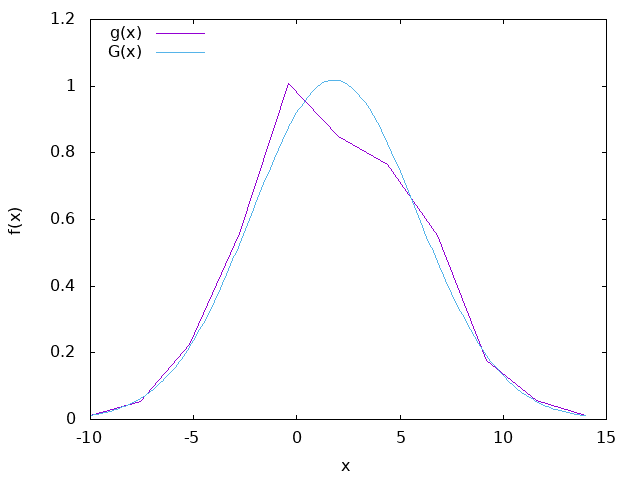
\includegraphics[width=10cm]{zaburzen.png}
\caption{Aproksymacja funkcji $g(x)$, parametr $\alpha=0, N=11$ węzłów aproksymacji}
\label{fig:obrazek zaburzen}
\end{figure}
Węzły znajdują się na linii funkcji, co jest zgodne ze sposobem w jaki sposób obliczane były wartości węzłów, jednak możemy zauważyć wystąpienie losowych szumów.
\begin{figure}[H]
\centering
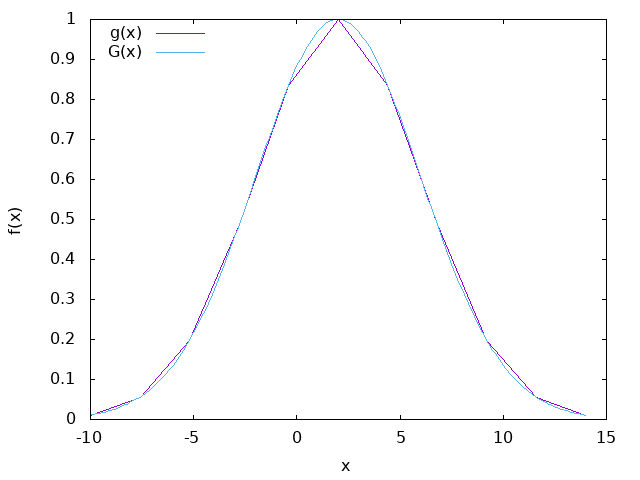
\includegraphics[width=10cm]{bez_zaburzen.png}
\caption{Aproksymacja funkcji g(x), parametr α = 0.5, N=11 węzłów aproksymacji}
\label{fig:obrazek bez_zaburzen}
\end{figure}

\begin{figure}[H]
\centering
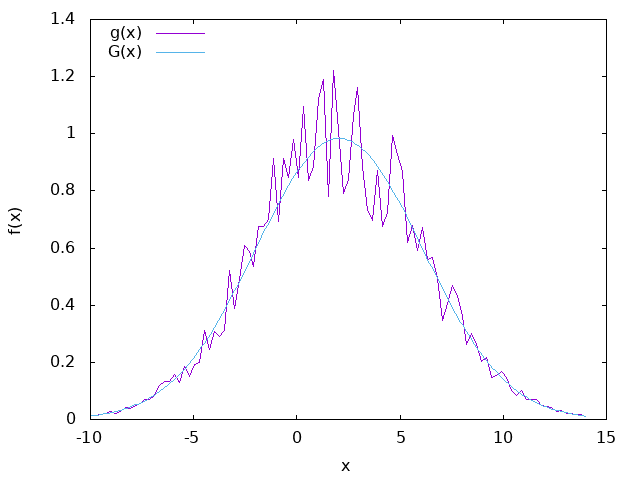
\includegraphics[width=10cm]{101.png}
\caption{Aproksymacja funkcji g(x), parametr α = 0.5, N=101 węzłów aproksymacji}
\label{fig:obrazek 101}
\end{figure}

\section{Wnioski}
Jak widać z powyższych wyników, aproksymacja funkcji bez szumu przy małej liczbie węzłów (N = 11)
idealnie pokrywa funkcję g(x). Aproksymacja wielomianowa pozwala na szybkie i dokładne wyznaczenie funkcji, gdy znamy jej wartości w
danym zbiorze. Jej dużą zaletą jest fakt, że do przybliżenia wartości funkcji nie potrzebny jest wielomian
wysokiego stopnia oraz fakt, że węzły mogą być równoodległe, a mimo to oszacowanie funkcji nie straci na
dokładności.
\end{document}